\message{ !name(AlgComplexAllFlashCards.tex)}\documentclass{beamer}
\title{Algorithms and Complexity, weeks 1-5 key points}
\author{Sam Barrett}
\newcommand{\qs}{q_{\texttt{start}}}
\newcommand{\qh}{q_{\texttt{halt}}}
\newcommand{\U}{\mathcal{U}}
\newcommand{\N}{\mathbb{N}}
\usepackage{mdframed,amsmath,amssymb,amsfonts,tikz}
\usetikzlibrary{shapes,arrows,calc,positioning,backgrounds}

\newmdtheoremenv{thesis}{Thesis}


\begin{document}

\message{ !name(AlgComplexAllFlashCards.tex) !offset(-3) }

\maketitle

\begin{frame}[allowframebreaks]
  \frametitle{Turing machine basics}

  \begin{itemize}
    \item Turing machines are \textbf{precise models of computation}
    \item First tape of a Turing machine is \textbf{always} a read-only \textbf{input tape}.
    \item The $k^{th}$ tape is always the output tape
    \item The output tape is also considered a work tape
    \item The alphabet of a TM is denoted as \(\Gamma\), it is \textbf{finite}.
    \item Each tape must always start with the \textit{left-of-tape} symbol, $\rhd$
    \item $\{ 0,1 \} ^{*}$ is the set of bitstrings, with $\varepsilon$ denoting the empty string.
  \end{itemize}

  \framebreak

  In a single stage of computation a TM may:
  \begin{itemize}
    \item reads the character at each tape head
    \item writes a character at each work tape head
    \item may move each tape head to the left or to the right. \textbf{note: our tapes are not recursive, if a head on the leftmost cell moves left, it stays put}
  \end{itemize}

\end{frame}

\begin{frame}
\frametitle{what does it mean to say that $M$ \textbf{computes} $f$?}

It means that for every bitstring $x \in \{ 0,1 \}^{*}$, if we start in state $\qs$ with the initial configuration showing $x$ (meaning $x$ appears on the input tape and and the work tapes are blank), when we run $M$, we eventually reach $\qh$ with the output tape showing $\rhd$ on the leftmost cell and then the bitstring $f(x)$ followed by all blanks.

\end{frame}

\begin{frame}
  \frametitle{Computable functions}
  \framesubtitle{Basics}

  \begin{definition}(Computable functions)
    We say a function $f : \{ 0,1 \} ^{*} \rightarrow \{ 0,1 \} ^{*}$ is \textbf{computable} if there exists some Turing machine that computes it and \textbf{non-computable} if there isn't.
  \end{definition}

  No variation of Turing machine affects this fact, giving us:

  \begin{thesis}(Church's Thesis)
    any algorithm that computes a function from bitstrings to bitstrings can be converted into a Turing machine that computes the same function
  \end{thesis}
\end{frame}

\begin{frame}[allowframebreaks]
  \frametitle{Boolean functions, languages and decidability}

  \begin{definition}
    A \textit{language} can be defined as any set of words
  \end{definition}

  \begin{definition}
    A \textbf{boolean function} is a function of the form: $f : \{ 0,1 \}^{*} \rightarrow \{ 0,1 \} $. Noting that the output is a single bit rather than a bitstring.
  \end{definition}

  There is a one-to-one correspondence between languages and boolean functions.
\begin{itemize}
  \item For a given boolean function $f$ the corresponding language is the set of bitstrings $x$ s.t. $f(x) = 1$
  \item For a language $L$, the corresponding boolean function sends $x$ to 1 if $x \in L$ and to $0$ otherwise.
\end{itemize}

This allows us to treat boolean functions, languages and decision problems as essentially the same thing.

A decision problem is said to be \textbf{decidable} when the corresponding boolean function is \textbf{computable}. I.e. given a language $L$, for $L$ to be decidable there must exist some Turing machine that will start with a bitstring $x$ and will run continuously until it halts and upon halting there will be a $1$ on the output tape if $x \in L$ or $0$ if it is not in the language.
\end{frame}

\begin{frame}
  \frametitle{Data Representation}
  \begin{itemize}
    \item We can encode many real-life data types as bitstrings, but not all. (e.g. Real numbers cannot)
    \item We can encode multiple inputs as a single bitstring.
  \end{itemize}
\end{frame}

\begin{frame}
  \frametitle{Code as Data}
  \begin{itemize}
    \item We can not only encode many data types as bitstrings, we can encode program code or even other Turing machines as bitstring inputs to a TM as our TMs are essentially 6-tuples (see full notes for formal definition).
    \item We can therefore say that for \textbf{any} bitstring \(\alpha\) we can construct a corresponding TM:  $M_{\alpha}$
  \end{itemize}
\end{frame}

\begin{frame}
  \frametitle{The Universal Turing Machine, $\U$}

  $\U$ is a Turing machine interpreter written as a Turing machine. It takes 2 inputs (encoded as a single input): $\alpha$ and $x$, where $\alpha$ is the bitstring describing the machine to be interpreted and $x$ is the bistring input.

  We define $\U$ as having 4 tapes and the basic alphabet of $\{ \rhd, \Box, 0,1 \} $.  Intuitively, $\U$ works by simulating the $M_{\alpha}$ by \textit{providing} it with the 3 non-input tapes to $M_{\alpha}$ as its input, work and output tape respectively.
\end{frame}

\begin{frame}[allowframebreaks]
  \frametitle{Diagonalisation \& the Halting problem}

  \begin{problem}(The halting problem)
    the set of pairs $\langle \alpha,x \rangle $ (encoded as a single bitstring) such that the machine $M_{\alpha}$ executed on input $x$ halts.
  \end{problem}

  \framebreak
  Turing's proof is as follows:

    \begin{proof}
    Suppose that $N$ is a machine that solves the halting problem.

    We can convert it into a machine $N'$ that, given $x$, runs forever if $\langle x,x \rangle \in \texttt{HALT} $ (i.e. the machine $M_{x}$ executed on $x$ halts), and halts otherwise.

    We know $N' = M_{\alpha }$ for some $\alpha $, i.e. there exists some bitstring $\alpha $ that represents our new machine, as we know every machine can be represented as a bitstring.

    Running $N'$ on $\alpha$ halts if it runs forever and runs forever if it halts.

    We have derived a contradiction.


  \end{proof}

  \framebreak

  More intuitively, we can consider the described machine $N$ as:
    \begin{center}
    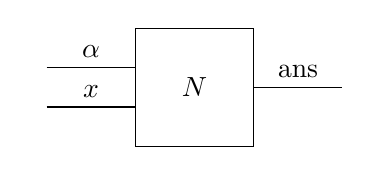
\begin{tikzpicture}

        \node [rectangle,draw,minimum size = 15mm] (N) at (2,2) {$N$};


        \node (i1) at (0,2.25) {};
        \node (i2) at (0,1.75) {};

        \draw (i1) -- node[above] {$\alpha $} (1.25,2.25);
        \draw (i2) -- node[above] {$x$} (1.25,1.75);

        \node (o1) at (4,2) {};

        \draw (N) -- node[above] {ans} (o1);
    \end{tikzpicture}
  \end{center}

  Where  \texttt{ans} is whether $N$ halts.

  We can then construct the wrapper $N'$ as:


    \begin{center}
    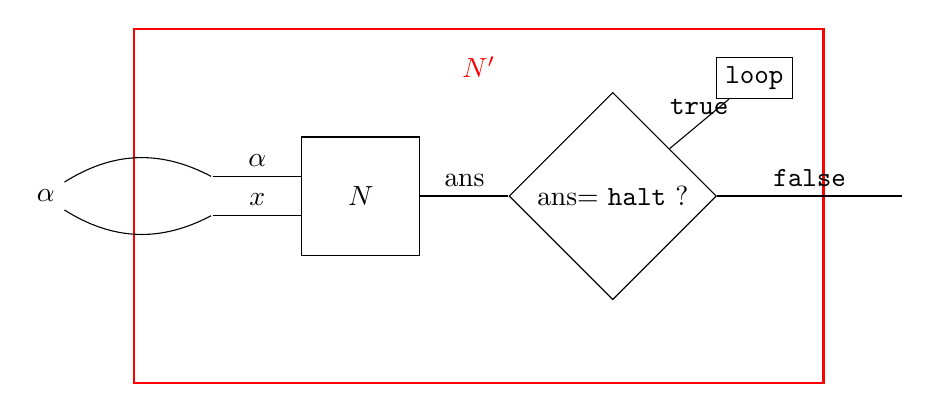
\begin{tikzpicture}
        %\draw [help lines] (-5,-5) grid (10,10);

        \node [rectangle,draw,minimum size = 15mm] (N) at (2,2) {$N$};


        \node (i1) at (0,2.25) {};
        \node (i2) at (0,1.75) {};

        \draw (i1) -- node[above] {$\alpha $} (1.25,2.25);
        \draw (i2) -- node[above] {$x$} (1.25,1.75);

        \node (o1) at (4,2) {};

        \draw (N) -- node[above] {ans} (o1);

        \draw[red,thick] ($(o1.north west)+(4,2)$)  rectangle node[above = 1.5cm of o1] {$N'$} ($(i2.south east)+(-1,-2)$);

        \node (i3) at (-2,2) {$\alpha $};

        \draw (i3) edge[bend right] (0.1,1.75);
        \draw (i3) edge[bend left] (0.1,2.25);
        \node [draw, diamond] (q) at (5.2,2){ans= \texttt{halt} ?};

        \node [draw,rectangle] (loop) at (7,3.5) {\texttt{loop} };

        \node (o2) at (9,2) {};

        \draw (q) -- node[above] {\texttt{false} } (o2);
        \draw (q) -- node[above] {\texttt{true} } (loop);


    \end{tikzpicture}
    \end{center}
    \textbf{Where the outermost $\alpha$ is the bitstring of $N'$}

    You can clearly see that if $N$ were to halt then $N'$ would hang. We can therefore derive a contradiction as if we pass $N'$ into $N'$ it would have to half if it hangs and vice versa!


  \end{frame}

  \begin{frame}
    \frametitle{Upper bound notation}

    \begin{itemize}
      \item     If we have two function $f : \N \rightarrow \N$ and $g : \N \rightarrow \N$
      \item We say that $f(n)$ is $O(g(n))$ is $f$ is \textbf{no bigger} than $g$ up to \textbf{a}  constant factor, i.e. given a constant $c$ and a value $n_{0}$ s.t. $\forall n, n \geq n_{0}$ we have:

            \[
            f(n) \leq c\cdot g(n)
            \]

      \item We say that $f(n)$ is $o(g(n))$ if $f$ is \textbf{not as big as }$g$, even up to any constant factor. Or, if, \textbf{for any} $\varepsilon > 0$, there is a $n_{0}$ s.t. $\forall n, n\geq n_{0}$ we have:

            \[
            f(n) \leq \varepsilon \cdot g(n)
            \]

            Whenever $f(n)$ is $o(g(n))$ is it also $O(g(n))$, this is the case if you take $c$ to be 1

    \end{itemize}


  \end{frame}

  \begin{frame}
    \frametitle{Lower bound notation}

    \begin{itemize}
      \item     If we have two function $f : \N \rightarrow \N$ and $g : \N \rightarrow \N$
      \item We say that $f(n)$ is $\Omega(g(n))$ when $g(n)$ is $O(f(n))$
      \item We say that $f(n)$ is $\omega(g(n))$ when $g(n)$ is $o(f(n))$
      \item We say that $f(n)$ is $\Theta(g(n))$ when it is \textbf{both} $O(g(n))$ and $\Omega(g(n))$

            This informally means \textit{$f(n)$ and $g(n)$ are the same, up to a constant factor}
    \end{itemize}
  \end{frame}
\end{document}

\message{ !name(AlgComplexAllFlashCards.tex) !offset(-242) }
